\documentclass[12pt,a4paper]{article}

% --- Page Layout -------------------------------------------------------------
\usepackage[a4paper, margin=0.8in, headheight=14pt]{geometry}

% --- Fonts (XeLaTeX) ---------------------------------------------------------
\usepackage{fontspec}
\usepackage{unicode-math}
\setmainfont{TeX Gyre Pagella}
\setmonofont[Scale=0.88]{TeX Gyre Cursor}
\setmathfont{Latin Modern Math}

% --- Packages ---------------------------------------------------------------
\usepackage{xcolor}
\usepackage{titlesec}
\usepackage{enumitem}
\usepackage{tabularx}
\usepackage{booktabs}
\usepackage{array}
\usepackage{amsmath}
\usepackage{tikz}
\usetikzlibrary{shapes.geometric, arrows.meta, positioning, calc, fit, decorations.pathreplacing}
\usepackage{tcolorbox}
\tcbuselibrary{skins, breakable}
\usepackage{hyperref}
\usepackage{fancyhdr}
\usepackage{graphicx}
\usepackage{microtype}
\hyphenpenalty=10000
\exhyphenpenalty=10000
\sloppy
\usepackage{caption}
\usepackage{setspace}
\usepackage{multirow}
\usepackage{tocloft}

% --- Q&A helper --------------------------------------------------------------
\newcommand{\Q}[1]{\textbf{#1}\par\noindent\ignorespaces}

% --- Colour Palette ----------------------------------------------------------
\definecolor{myred}{RGB}{196,30,58}
\definecolor{mydark}{RGB}{30,30,50}
\definecolor{mygreen}{RGB}{14,120,80}
\definecolor{myteal}{RGB}{0,130,140}
\definecolor{myamber}{RGB}{180,100,0}
\definecolor{mypurple}{RGB}{100,30,160}
\definecolor{mygray}{RGB}{246,247,249}
\definecolor{mgframe}{RGB}{180,185,200}
\definecolor{watermark}{RGB}{145,150,170}
\definecolor{hdrred}{RGB}{250,232,235}
\definecolor{hdrgreen}{RGB}{220,244,233}
\definecolor{hdrteal}{RGB}{220,242,244}
\definecolor{hdramber}{RGB}{253,242,215}
\definecolor{hdrpurple}{RGB}{238,228,255}

% --- Section Formatting ------------------------------------------------------
\titleformat{\section}
  {\large\bfseries\color{myred}}{\thesection.}{0.5em}{}
  [\vspace{1pt}{\color{myred}\rule{\linewidth}{0.8pt}}]
\titleformat{\subsection}
  {\normalsize\bfseries\color{myteal}}{\thesubsection}{0.5em}{}
\titlespacing*{\section}{0pt}{18pt}{7pt}
\titlespacing*{\subsection}{0pt}{11pt}{4pt}

% --- Paragraph ---------------------------------------------------------------
\setlength{\parindent}{0pt}
\setlength{\parskip}{4pt}

% --- TOC Styling -------------------------------------------------------------
\renewcommand{\cfttoctitlefont}{\large\bfseries\color{myred}}
\renewcommand{\cftaftertoctitle}{\par\noindent{\color{myred}\rule{\linewidth}{0.8pt}}}
\setlength{\cftbeforetoctitleskip}{0pt}
\setlength{\cftaftertoctitleskip}{6pt}
\renewcommand{\cftsecfont}{\normalsize\bfseries\color{mydark}}
\renewcommand{\cftsecpagefont}{\normalsize\bfseries\color{mydark}}
\renewcommand{\cftsecleader}{\cftdotfill{\cftdotsep}}
\setlength{\cftbeforesecskip}{7pt}
\renewcommand{\cftsubsecfont}{\small\color{mydark}}
\renewcommand{\cftsubsecpagefont}{\small\color{mydark}}
\setlength{\cftbeforesubsecskip}{3pt}
\setlength{\cftsubsecindent}{1.4em}

% --- Table helpers -----------------------------------------------------------
\renewcommand{\arraystretch}{1.45}
\setlength{\tabcolsep}{6pt}
\newcolumntype{B}[1]{>{\small\bfseries\raggedright\arraybackslash}m{#1}}
\newcolumntype{Y}{>{\small\raggedright\arraybackslash}X}
\renewcommand{\tabularxcolumn}[1]{m{#1}}

% --- Header / Footer ---------------------------------------------------------
\pagestyle{fancy}
\fancyhf{}
\fancyhead[L]{\small\color{myred}\textbf{BS-PH101}\;\color{mydark}--- Physics-I}
\fancyhead[R]{\small\color{myteal}\textbf{Module 2 Notes}}
\fancyfoot[C]{\small\color{mydark}\thepage}
\fancyfoot[R]{\small\color{watermark}\textit{\copyright\ Biraj}}
\renewcommand{\headrulewidth}{0.5pt}
\renewcommand{\footrulewidth}{0.3pt}

% --- Hyperref ---------------------------------------------------------------
\hypersetup{
  colorlinks=true, linkcolor=myteal, urlcolor=myteal,
  pdfauthor={Biraj Sarkar},
  pdftitle={BS-PH101 --- Module 2 Notes}
}

% --- tcolorbox styles --------------------------------------------------------
\tcbset{
  tikzbox/.style={
    colback=mygray, colframe=mgframe, boxrule=0.6pt, arc=4pt,
    left=8pt, right=8pt, top=6pt, bottom=6pt,
    colbacktitle=mgframe, coltitle=mydark, fonttitle=\small\bfseries
  },
  defbox/.style={
    colback=hdrgreen, colframe=mygreen, boxrule=0.8pt, arc=4pt,
    left=9pt, right=9pt, top=6pt, bottom=6pt,
    colbacktitle=mygreen, coltitle=white, fonttitle=\small\bfseries
  },
  formulabox/.style={
    colback=hdrteal, colframe=myteal, boxrule=0.8pt, arc=4pt,
    left=9pt, right=9pt, top=7pt, bottom=7pt,
    colbacktitle=myteal, coltitle=white, fonttitle=\small\bfseries
  },
  examplebox/.style={
    colback=hdramber, colframe=myamber, boxrule=0.8pt, arc=4pt,
    left=9pt, right=9pt, top=6pt, bottom=6pt,
    colbacktitle=myamber, coltitle=white, fonttitle=\small\bfseries
  },
  masonbox/.style={
    colback=hdrpurple, colframe=mypurple, boxrule=0.8pt, arc=4pt,
    left=9pt, right=9pt, top=6pt, bottom=6pt,
    colbacktitle=mypurple, coltitle=white, fonttitle=\small\bfseries
  },
  exambox/.style={
    colback=hdrpurple, colframe=mypurple, boxrule=1pt, arc=5pt,
    left=10pt, right=10pt, top=8pt, bottom=8pt,
    colbacktitle=mypurple, coltitle=white, fonttitle=\bfseries,
    breakable, title after break={\textbf{Frequently Asked / Viva Questions (contd.)}}
  }
}
\tcbset{breakable}

% --- TikZ Styles -------------------------------------------------------------
\tikzset{
  block/.style={rectangle, draw=myteal, fill=hdrteal, text width=2.4cm, align=center, minimum height=0.95cm, font=\small, rounded corners=3pt, line width=0.7pt},
  redblock/.style={rectangle, draw=myred, fill=hdrred, text width=2.4cm, align=center, minimum height=0.95cm, font=\small, rounded corners=3pt, line width=0.7pt},
  arrow/.style={-Stealth, thick, color=mydark},
  redarrow/.style={-Stealth, thick, color=myred},
  line/.style={thick, color=mydark}
}

\begin{document}

% --- Title Page --------------------------------------------------------------
\begin{center}
  {\LARGE\bfseries\color{myred} BS-PH101 --- Physics-I}\\[5pt]
  {\normalsize\color{mydark} Semester I/II \quad$\bullet$\quad 3L:1T:0P \quad$\bullet$\quad 4 Credits}\\[3pt]
  {\normalsize\color{myteal}\textbf{Module 2 Comprehensive Exam Notes: Optics}}\\[3pt]
  {\small\color{mydark} CGEC \;$|$\; B.Tech ECE (2023--27) \;$|$\; \textit{Biraj Sarkar}}
\end{center}
\vspace{2pt}
\noindent{\color{myred}\rule{\linewidth}{1.5pt}}
\vspace{2pt}
\hypersetup{linkcolor=mydark}
\tableofcontents
\hypersetup{linkcolor=myteal}
\newpage

% =============================================================================
% SECTION 1: INTERFERENCE VS DIFFRACTION
% =============================================================================
\section{Interference vs. Diffraction and Classification}

\subsection{Distinction Between Interference and Diffraction}

\begin{tcolorbox}[defbox, title={\textbf{Definition: Interference and Diffraction}}]
\begin{itemize}[leftmargin=*, itemsep=2pt]
  \item \textbf{Interference:} Modification in intensity resulting from the superposition of two or more coherent light waves originating from distinct coherent sources.
  \item \textbf{Diffraction:} The bending of light waves around the sharp edges of an obstacle or aperture and their subsequent superposition within the geometrical shadow region.
\end{itemize}
\end{tcolorbox}

\textbf{Comprehensive Comparison:}\par\vspace{6pt}\noindent
\begin{tabularx}{\linewidth}{|B{3.2cm}|Y|Y|}
\hline
\textbf{Property} & \textbf{Interference} & \textbf{Diffraction} \\
\hline
\textbf{Wave Origin} & Superposition of waves from two distinct coherent sources. & Superposition of secondary wavelets originating from different points of the \textit{same} wavefront. \\
\hline
\textbf{Fringe Width} & Fringes are usually of equal width ($\beta = \lambda D / d$). & Fringes are never of equal width (central max is twice as wide as secondary max). \\
\hline
\textbf{Intensity} & All bright fringes have equal intensity ($I_{\max} = 4 I_0$). & Intensity decreases rapidly with increasing order of secondary maxima. \\
\hline
\textbf{Darkness} & Minima are completely dark ($I_{\min} = 0$). & Minima are generally not completely dark. \\
\hline
\end{tabularx}

\subsection{Fraunhofer vs. Fresnel Diffraction}

\begin{tabularx}{\linewidth}{|B{3.2cm}|Y|Y|}
\hline
\textbf{Feature} & \textbf{Fresnel Diffraction} & \textbf{Fraunhofer Diffraction} \\
\hline
\textbf{Distance} & Source and screen are at finite distances from aperture. & Source and screen are at effectively infinite distances. \\
\hline
\textbf{Wavefront} & Incident wavefront is spherical or cylindrical. & Incident wavefront is plane (parallel rays). \\
\hline
\textbf{Lenses} & No lenses required to focus pattern. & Convex lenses required before and after aperture. \\
\hline
\textbf{Analysis} & Analyzed using Fresnel half-period zones. & Analyzed using simple wave phase summation. \\
\hline
\end{tabularx}

% =============================================================================
% SECTION 2: FRAUNHOFER DIFFRACTION
% =============================================================================
\section{Fraunhofer Diffraction at Single, Double, and Multiple Slits}

\subsection{Single Slit Diffraction}

Consider a plane wavefront of wavelength $\lambda$ incident normally on a slit of width $e$.

\begin{tcolorbox}[formulabox, title={\textbf{Single Slit Intensity Formula}}]
The resultant intensity on a screen at diffraction angle $\theta$ is:
\begin{equation}
I(\theta) = I_0 \left(\frac{\sin \beta}{\beta}\right)^2 \quad \text{where } \beta = \frac{\pi e \sin \theta}{\lambda}
\end{equation}
\end{tcolorbox}

\textbf{Key Conditions:}\par\noindent
\begin{itemize}[leftmargin=*, itemsep=3pt]
  \item \textbf{Central Maximum:} At $\theta = 0 \implies \beta = 0$, $\lim_{\beta\to 0} \frac{\sin\beta}{\beta} = 1 \implies I = I_0$.
  \item \textbf{Minima Condition:} $\sin \beta = 0$ (for $\beta \neq 0$) $\implies \beta = m \pi \implies e \sin \theta = m \lambda \quad (m = \pm 1, \pm 2, \pm 3, \ldots)$.
  \item \textbf{Secondary Maxima:} Occur near $\beta = \pm 1.43 \pi, \pm 2.46 \pi, \dots$ with intensity ratios:
  \begin{equation}
  I_0 : I_1 : I_2 = 1 : \frac{1}{22} : \frac{1}{61} = 1 : 0.045 : 0.016
  \end{equation}
  \item \textbf{Width of Central Maximum:} $\Delta \theta = \frac{2 \lambda}{e} \implies \text{Linear Width } W = \frac{2 \lambda f}{e}$ (where $f$ is lens focal length).
\end{itemize}

\subsection{Double Slit Diffraction}

For two parallel slits, each of width $e$ and separated by opaque spacing $d$ (grating element $= e + d$):

\begin{tcolorbox}[formulabox, title={\textbf{Double Slit Intensity Formula}}]
\begin{equation}
I(\theta) = 4 I_0 \left(\frac{\sin \beta}{\beta}\right)^2 \cos^2 \alpha \quad \text{where } \beta = \frac{\pi e \sin \theta}{\lambda}, \;\; \alpha = \frac{\pi (e+d) \sin \theta}{\lambda}
\end{equation}
It is the product of single-slit diffraction factor $\left(\frac{\sin\beta}{\beta}\right)^2$ and interference factor $\cos^2\alpha$.
\end{tcolorbox}

\textbf{Missing Orders (Absent Spectra):} Occurs when an interference maximum coincides with a diffraction minimum:
\begin{equation}
(e+d)\sin\theta = n \lambda \quad \text{and} \quad e\sin\theta = m \lambda \implies \frac{e+d}{e} = \frac{n}{m}
\end{equation}
If $e = d$, then $\frac{n}{m} = 2 \implies n = 2m$, so $2^{\text{nd}}, 4^{\text{th}}, 6^{\text{th}}$ interference orders disappear.

\subsection{Diffraction Grating and Resolving Power}

A plane transmission diffraction grating consists of $N$ parallel, equally spaced slits with grating element $(e+d)$.

\begin{tcolorbox}[formulabox, title={\textbf{Grating Equations and Resolving Power}}]
\begin{itemize}[leftmargin=*, itemsep=3pt]
  \item \textbf{Principal Maxima Condition:}
  \begin{equation}
  (e+d)\sin\theta = m \lambda \quad (m = 0, 1, 2, \ldots)
  \end{equation}
  \item \textbf{Dispersive Power ($D$):} Rate of change of diffraction angle with wavelength:
  \begin{equation}
  D = \frac{d\theta}{d\lambda} = \frac{m}{(e+d)\cos\theta}
  \end{equation}
  \item \textbf{Resolving Power ($R$):} Capacity to separate two spectral lines of wavelength $\lambda$ and $\lambda + d\lambda$:
  \begin{equation}
  R = \frac{\lambda}{d\lambda} = m N \quad (N = \text{total illuminated rulings})
  \end{equation}
\end{itemize}
\end{tcolorbox}

\begin{tcolorbox}[examplebox, title={\textbf{Solved Problem 1: Grating Spectral Lines and Maximum Order}}]
\textbf{Problem:} A grating has $5000\text{ lines/cm}$. Light of wavelength $\lambda = 6000\text{ \AA}$ is incident normally. Find: (a) Grating element $(e+d)$, (b) Highest observable order.

\textbf{Solution:}\par\noindent
\begin{enumerate}[leftmargin=*, itemsep=2pt]
  \item Grating element $(e+d) = \frac{1\text{ cm}}{5000} = 2 \times 10^{-4}\text{ cm} = 2 \times 10^{-6}\text{ m}$.
  \item Maximum angle $\theta_{\max} = 90^\circ \implies \sin 90^\circ = 1$.
  \item Substitute in grating equation $(e+d)\sin 90^\circ = m_{\max} \lambda$:
   \begin{equation}
   m_{\max} = \frac{(e+d)}{\lambda} = \frac{2 \times 10^{-6}\text{ m}}{600 \times 10^{-9}\text{ m}} = 3.33 \implies \mathbf{m_{\max} = 3}
   \end{equation}
\end{enumerate}
Hence, maximum $3^{\text{rd}}$ order spectrum can be observed.
\end{tcolorbox}

\begin{tcolorbox}[examplebox, title={\textbf{Solved Problem 2: Single Slit Central Width}}]
\textbf{Problem:} Light of wavelength $\lambda = 5890\text{ \AA}$ is incident normally on a slit of width $0.1\text{ mm}$. A convex lens of focal length $f = 1.0\text{ m}$ is placed behind the slit. Calculate linear width of central maximum.

\textbf{Solution:}\par\noindent
Linear width of central maximum $W = \frac{2 \lambda f}{e}$.
$W = \frac{2 \times 5890 \times 10^{-10}\text{ m} \times 1.0\text{ m}}{0.1 \times 10^{-3}\text{ m}} = 11.78 \times 10^{-3}\text{ m} = \mathbf{11.78\text{ mm}}$.
\end{tcolorbox}

% =============================================================================
% SECTION 3: POLARISATION OF LIGHT
% =============================================================================
\section{Polarisation of Light}

\subsection{Brewster's Law and Double Refraction}

\begin{tcolorbox}[defbox, title={\textbf{Brewster's Law}}]
When unpolarised light is incident at a specific angle $i_p$ (polarising angle) on a dielectric interface, the reflected light is $100\%$ plane polarised with electric vector perpendicular to plane of incidence.
\begin{equation}
\mu = \tan i_p \quad \text{and} \quad i_p + r = 90^\circ
\end{equation}
\end{tcolorbox}

\begin{tcolorbox}[tikzbox, title={Polarisation by Reflection (Brewster's Law)}]
\centering
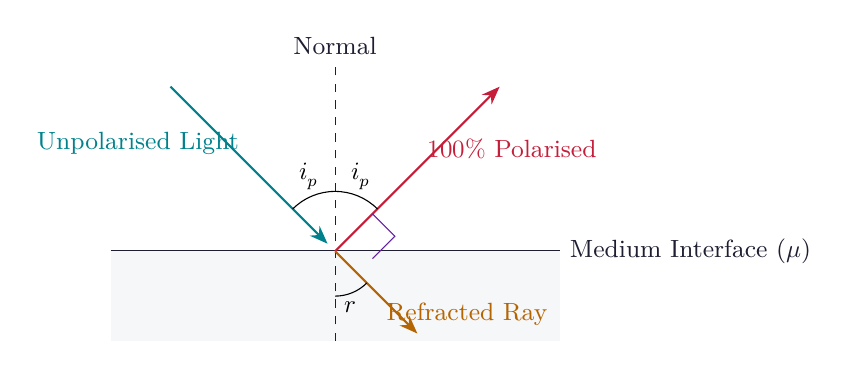
\begin{tikzpicture}[scale=0.95]
  % Boundary
  \draw[thick, mydark] (-3,0) -- (3,0) node[right] {\small Medium Interface ($\mu$)};
  \fill[mygray] (-3,-1.2) rectangle (3,0);
  
  % Normal
  \draw[dashed, mydark] (0,-1.2) -- (0,2.5) node[above] {\small Normal};
  
  % Rays
  \draw[thick, myteal, -Stealth] (-2.2,2.2) -- (-0.1,0.1) node[midway, above left] {\small Unpolarised Light};
  \draw[thick, myred, -Stealth] (0,0) -- (2.2,2.2) node[midway, above right] {\small $100\%$ Polarised};
  \draw[thick, myamber, -Stealth] (0,0) -- (1.1,-1.1) node[midway, below right] {\small Refracted Ray};
  
  % Angles
  \draw[thin] (0,0.8) arc (90:135:0.8);
  \node at (-0.35,1.0) {\small $i_p$};
  \draw[thin] (0,0.8) arc (90:45:0.8);
  \node at (0.35,1.0) {\small $i_p$};
  \draw[thin] (0,-0.6) arc (270:315:0.6);
  \node at (0.2,-0.75) {\small $r$};
  
  % 90 deg marker between reflected and refracted
  \draw[thin, mypurple] (0.5,0.5) -- (0.8,0.2) -- (0.5,-0.1);
\end{tikzpicture}
\end{tcolorbox}

\textbf{Double Refraction (Birefringence):} When unpolarised light enters an anisotropic crystal (e.g. Calcite, Quartz), it splits into two plane polarised rays travelling at different speeds:
\begin{itemize}[leftmargin=*, itemsep=2pt]
  \item \textbf{Ordinary Ray ($O$-ray):} Obeys Snell's law; travels with equal velocity in all directions ($v_o = c/\mu_o$).
  \item \textbf{Extraordinary Ray ($E$-ray):} Violates Snell's law; velocity depends on direction of propagation ($v_e$).
\end{itemize}

\subsection{Retardation Plates: Quarter-Wave and Half-Wave Plates}

\begin{tcolorbox}[formulabox, title={\textbf{Retardation Plate Thickness Equations}}]
For a crystal plate cut parallel to optic axis of thickness $t$:
\begin{itemize}[leftmargin=*, itemsep=3pt]
  \item \textbf{Quarter-Wave Plate (QWP):} Introduces phase difference $\Delta \phi = \pi/2$ or path difference $\Delta x = \lambda/4$:
  \begin{equation}
  t = \frac{\lambda}{4 |\mu_o - \mu_e|}
  \end{equation}
  \item \textbf{Half-Wave Plate (HWP):} Introduces phase difference $\Delta \phi = \pi$ or path difference $\Delta x = \lambda/2$:
  \begin{equation}
  t = \frac{\lambda}{2 |\mu_o - \mu_e|}
  \end{equation}
\end{itemize}
\end{tcolorbox}

\subsection{Optical Activity and Laurent's Half-Shade Polarimeter}

Optically active substances rotate the plane of polarization of linearly polarized light.
The angle of rotation $\theta$ is given by Biot's law: $\theta = S \cdot L \cdot c$.
\begin{equation}
\text{Specific Rotation } [S]_\lambda^T = \frac{\theta}{L \cdot c} \quad \left(\text{in } \frac{\text{deg}}{\text{dm} \cdot \text{g/cm}^3}\right)
\end{equation}
where $\theta = \text{rotation angle (deg)}$, $L = \text{path length in decimeters (dm)}$, $c = \text{concentration in g/cm}^3$.

\textbf{Laurent's Half-Shade Polarimeter:} Uses a half-shade plate (half quartz, half glass) to divide the field of view into two halves, enabling precise setting of equal brightness.

\begin{tcolorbox}[examplebox, title={\textbf{Solved Problem 3: Quarter-Wave Plate Thickness}}]
\textbf{Problem:} Calculate the minimum thickness of a quarter-wave plate of Calcite for sodium light of wavelength $\lambda = 5893\text{ \AA}$. Given $\mu_o = 1.6583$ and $\mu_e = 1.4864$.

\textbf{Solution:}\par\noindent
\begin{enumerate}[leftmargin=*, itemsep=2pt]
  \item Calcite is a negative crystal ($\mu_o > \mu_e$), so $|\mu_o - \mu_e| = 1.6583 - 1.4864 = 0.1719$.
  \item Formula: $t = \frac{\lambda}{4(\mu_o - \mu_e)}$.
  \item Substitute: $t = \frac{5893 \times 10^{-10}\text{ m}}{4 \times 0.1719} = \frac{5893 \times 10^{-10}}{0.6876} = 8570 \times 10^{-10}\text{ m} = \mathbf{0.857\text{ \mu m}}$.
\end{enumerate}
\end{tcolorbox}

% =============================================================================
% SECTION 4: LASERS
% =============================================================================
\section{Lasers (Light Amplification by Stimulated Emission of Radiation)}

\subsection{Principles of Laser Action: Einstein's Coefficients}

Interaction of radiation with matter involves three fundamental processes:

\begin{tcolorbox}[formulabox, title={\textbf{Three Radiation Processes and Einstein's Relations}}]
\begin{enumerate}[leftmargin=*, itemsep=3pt]
  \item \textbf{Stimulated Absorption:} Atom absorbs photon: Rate $R_{12} = B_{12} N_1 u(\nu)$.
  \item \textbf{Spontaneous Emission:} Atom decays naturally: Rate $R_{21,\text{sp}} = A_{21} N_2$.
  \item \textbf{Stimulated Emission:} Incident photon induces decay: Rate $R_{21,\text{st}} = B_{21} N_2 u(\nu)$.
\end{enumerate}
At thermal equilibrium, $R_{12} = R_{21,\text{sp}} + R_{21,\text{st}}$. Equating with Planck's law yields Einstein's relations:
\begin{equation}
B_{12} = B_{21} \quad \text{and} \quad \frac{A_{21}}{B_{21}} = \frac{8\pi h \nu^3}{c^3}
\end{equation}
\end{tcolorbox}

\subsection{Population Inversion and Pumping}

Under normal thermal equilibrium (Boltzmann distribution $N_2 = N_1 e^{-h\nu/kT}$), $N_1 \gg N_2$.

\begin{tcolorbox}[defbox, title={\textbf{Definition: Population Inversion and Pumping}}]
\begin{itemize}[leftmargin=*, itemsep=2pt]
  \item \textbf{Population Inversion:} The non-equilibrium state in which higher energy level population exceeds lower energy level ($N_2 > N_1$). Necessary condition for optical amplification.
  \item \textbf{Pumping:} The external process of supplying energy to raise atoms to higher excited levels to achieve population inversion (e.g. Optical pumping, Electrical discharge, Direct electron excitation).
  \item \textbf{Metastable State:} An excited state with a long lifetime ($\sim 10^{-3}\text{ s}$ compared to normal $10^{-8}\text{ s}$), allowing accumulation of atoms for population inversion.
\end{itemize}
\end{tcolorbox}

\subsection{He-Ne Laser (Gas Laser)}

\begin{tcolorbox}[tikzbox, title={He-Ne Laser Energy Level Diagram}]
\centering
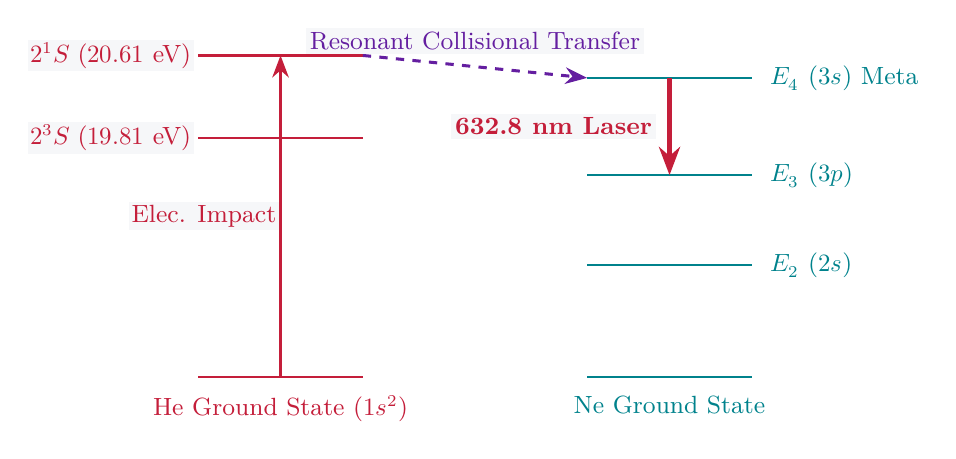
\begin{tikzpicture}[scale=0.95]
  % He Levels (Left)
  \draw[thick, myred] (0.6,0) -- (2.8,0) node[midway, below=3pt] {\small He Ground State ($1s^2$)};
  \draw[thick, myred] (0.6,3.2) -- (2.8,3.2);
  \node[myred, fill=mygray, inner sep=1pt, anchor=east] at (0.55, 3.2) {\small $2^3S$ ($19.81\text{ eV}$)};
  
  \draw[thick, myred] (0.6,4.3) -- (2.8,4.3);
  \node[myred, fill=mygray, inner sep=1pt, anchor=east] at (0.55, 4.3) {\small $2^1S$ ($20.61\text{ eV}$)};
  
  % Ne Levels (Right)
  \draw[thick, myteal] (5.8,0) -- (8.0,0) node[midway, below=3pt] {\small Ne Ground State};
  \draw[thick, myteal] (5.8,1.5) -- (8.0,1.5) node[right=3pt] {\small $E_2$ ($2s$)};
  \draw[thick, myteal] (5.8,2.7) -- (8.0,2.7) node[right=3pt] {\small $E_3$ ($3p$)};
  \draw[thick, myteal] (5.8,4.0) -- (8.0,4.0) node[right=3pt] {\small $E_4$ ($3s$) Meta};
  
  % Excitation & Transfer
  \draw[-Stealth, redarrow, line width=1.1pt] (1.7,0) -- (1.7,4.3) node[midway, fill=mygray, inner sep=1pt, anchor=east] {\small Elec. Impact};
  \draw[-Stealth, dashed, line width=1.1pt, mypurple] (2.8,4.3) -- (5.8,4.0) node[midway, above=4pt, fill=mygray, inner sep=1.5pt] {\small Resonant Collisional Transfer};
  
  % Laser Transition (Arrow on right, text on left of arrow)
  \draw[-Stealth, line width=1.6pt, myred] (6.9,4.0) -- (6.9,2.7) node[midway, left=4pt, fill=mygray, inner sep=1.5pt] {\small\textbf{632.8 nm Laser}};
\end{tikzpicture}
\end{tcolorbox}

\textbf{Working Mechanism of He-Ne Laser:}
\begin{enumerate}[leftmargin=*, itemsep=2pt]
  \item Electric discharge accelerates electrons which excite He atoms to metastable $2^1S$ ($20.61\text{ eV}$) state.
  \item He atoms transfer energy to Ne atoms via resonant inelastic collisions, populating Ne's $3s$ ($E_4$) level.
  \item Stimulated emission from $3s \to 2p$ ($E_4 \to E_3$) produces red laser light at $\lambda = 632.8\text{ nm}$.
\end{enumerate}

% =============================================================================
% QUICK REVISION PAGE
% =============================================================================
\newpage
\begin{center}
  {\large\bfseries\color{myred} Quick Revision --- Module 2}\\[3pt]
  {\small\color{mydark} Optics $|$ BS-PH101}
\end{center}
\noindent{\color{myred}\rule{\linewidth}{1.2pt}}
\vspace{4pt}

\begin{tcolorbox}[formulabox, title={\textbf{Key Formulas and Metrics at a Glance}}]
\renewcommand{\arraystretch}{1.35}
\begin{tabularx}{\linewidth}{B{5.0cm} X}
Single Slit Minima & $e \sin\theta = m \lambda \quad (m = \pm 1, \pm 2, \ldots)$ \\[4pt]
Single Slit Central Width & $\Delta \theta = \frac{2\lambda}{e} \implies \text{Linear Width } W = \frac{2\lambda f}{e}$ \\[4pt]
Double Slit Missing Orders & $\frac{e+d}{e} = \frac{n}{m} \quad (n = \text{interf. order}, m = \text{diff. order})$ \\[4pt]
Grating Equation & $(e+d)\sin\theta = m \lambda$ \\[4pt]
Grating Dispersive Power & $D = \frac{d\theta}{d\lambda} = \frac{m}{(e+d)\cos\theta}$ \\[4pt]
Grating Resolving Power & $R = \frac{\lambda}{d\lambda} = m N$ \\[4pt]
Brewster's Law & $\mu = \tan i_p \quad \text{and} \quad i_p + r = 90^\circ$ \\[4pt]
Quarter-Wave Plate (QWP) & $t = \frac{\lambda}{4 |\mu_o - \mu_e|}$ \\[4pt]
Half-Wave Plate (HWP) & $t = \frac{\lambda}{2 |\mu_o - \mu_e|}$ \\[4pt]
Specific Rotation & $[S]_\lambda^T = \frac{\theta}{L \cdot c} \quad (\text{deg} \cdot \text{dm}^{-1} \cdot (\text{g/cm}^3)^{-1})$ \\[4pt]
Einstein Coefficients Relation & $\frac{A_{21}}{B_{21}} = \frac{8\pi h \nu^3}{c^3} \quad \text{and} \quad B_{12} = B_{21}$ \\[4pt]
\end{tabularx}
\end{tcolorbox}

\begin{tcolorbox}[defbox, title={\textbf{One-Line Definitions}}]
\begin{itemize}[leftmargin=*, itemsep=2pt]
  \item \textbf{Diffraction Grating:} An optical component with a periodic structure of $N$ slits that diffracts light into several beams.
  \item \textbf{Brewster Angle ($i_p$):} Angle of incidence at which light with a particular polarization is perfectly transmitted without reflection.
  \item \textbf{Birefringence:} The optical property of a material having a refractive index that depends on the polarization and propagation direction of light.
  \item \textbf{Population Inversion:} State in which a system exists with more members in an excited state than in lower energy states ($N_2 > N_1$).
  \item \textbf{Metastable State:} An excited atomic state with a long lifetime ($\sim 10^{-3}\text{ s}$), essential for building up population inversion.
\end{itemize}
\end{tcolorbox}

\begin{tcolorbox}[exambox, title={\textbf{Frequently Asked / Viva Questions}}]
\begin{enumerate}[topsep=0pt, label=\textbf{Q\arabic*.}, itemsep=5pt]
  \item \Q{What is the basic difference between interference and diffraction?}
  Interference results from superposition of waves from two distinct coherent sources; diffraction results from superposition of wavelets from different parts of the same wavefront.

  \item \Q{Why is central maximum in single-slit diffraction twice as wide as secondary maxima?}
  Because central maximum extends between first minima on either side ($\sin\theta = \pm \lambda/e$), spanning angular width $2\lambda/e$, whereas secondary maxima span width $\lambda/e$.

  \item \Q{What is meant by missing orders in double slit diffraction?}
  Missing orders occur when an interference maximum coincides with a diffraction minimum at the same angle $\theta$, making that order absent ($\frac{e+d}{e} = \frac{n}{m}$).

  \item \Q{State Rayleigh's criterion for spectral resolution.}
  Two spectral lines are just resolved when the central principal maximum of one falls on the first minimum of the other.

  \item \Q{How does resolving power of a grating differ from dispersive power?}
  Dispersive power ($d\theta/d\lambda$) measures angular separation between lines; resolving power ($\lambda/d\lambda = mN$) measures ability to distinguish two close wavelengths.

  \item \Q{State Brewster's law and show reflected and refracted rays are perpendicular.}
  $\mu = \tan i_p$. Since $\frac{\sin i_p}{\sin r} = \tan i_p = \frac{\sin i_p}{\cos i_p} \implies \sin r = \cos i_p = \sin(90^\circ - i_p) \implies i_p + r = 90^\circ$.

  \item \Q{What are $O$-ray and $E$-ray in a birefringent crystal?}
  $O$-ray (Ordinary) obeys Snell's law with constant speed $v_o$; $E$-ray (Extraordinary) violates Snell's law with directional speed $v_e$.

  \item \Q{Distinguish between positive and negative uniaxial crystals.}
  In positive crystals ($\mu_e > \mu_o$, e.g. Quartz), $v_o > v_e$; in negative crystals ($\mu_o > \mu_e$, e.g. Calcite), $v_e > v_o$.

  \item \Q{Explain the function of a Quarter-Wave Plate (QWP).}
  A QWP introduces a path difference of $\lambda/4$ ($\pi/2$ phase shift) between $O$-ray and $E$-ray, converting linearly polarized light to circularly or elliptically polarized light.

  \item \Q{What is population inversion and why is it necessary for laser action?}
  Population inversion ($N_2 > N_1$) ensures that rate of stimulated emission exceeds rate of stimulated absorption, producing net optical amplification.

  \item \Q{Why is Helium gas added to Neon gas in a He-Ne laser?}
  He atoms are excited by electron impact to metastable states ($2^1S, 2^3S$) and efficiently transfer energy to Ne atoms via resonant collisions, achieving population inversion in Ne.

  \item \Q{Derive relation between Einstein $A$ and $B$ coefficients.}
  Equating thermal equilibrium rate $B_{12} N_1 u(\nu) = A_{21} N_2 + B_{21} N_2 u(\nu)$ with Boltzmann distribution $N_2/N_1 = e^{-h\nu/kT}$ and Planck's radiation law gives $B_{12} = B_{21}$ and $A_{21}/B_{21} = 8\pi h\nu^3/c^3$.
\end{enumerate}
\end{tcolorbox}

\begin{tcolorbox}[tikzbox, title={Summary Comparison of Laser Processes}]
\centering
\begin{tabularx}{\linewidth}{|B{3.2cm}|Y|Y|Y|}
\hline
\textbf{Process} & \textbf{Incident Condition} & \textbf{Transition} & \textbf{Output Properties} \\
\hline
\textbf{Absorption} & Photon ($h\nu = E_2 - E_1$) & Lower $E_1 \to$ Higher $E_2$ & Atom reaches excited state. \\
\hline
\textbf{Spontaneous Emission} & Natural decay (lifetime $\sim 10^{-8}\text{s}$) & Higher $E_2 \to$ Lower $E_1$ & Incoherent, random phase/direction. \\
\hline
\textbf{Stimulated Emission} & Triggering photon ($h\nu$) & Higher $E_2 \to$ Lower $E_1$ & Coherent, identical phase, direction, and wavelength. \\
\hline
\end{tabularx}
\end{tcolorbox}

\end{document}
